

Several backgrounds to the signal are simulated purely using MC simulation.
The details of these processes, like why they function as backgrounds
to the signal and which MC generators are used in the simulation,
have already been described in \sec\ref{sec:www_bg_samples}.
In some cases, corrections and/or uncertainties on 
the normalization of these simulated samples are applied. 
The corrections are summarized in \tab\ref{tab:mcnorm} and are described
in more detail below.
Those simulated backgrounds
which are most important have been checked in control regions and are 
also described below.

\begin{table}[htp]
\centering
    \begin{tabular}{|c|cc|}
    \hline
    Background & Normalization Factor & Uncertainty \\ 
    \hline\hline
    $WZ$ & 1.08 & 10~\% \\
    $ZZ$ & 1.05 & 15~\% \\
    %$Z\gamma$ & & 30~\% \\
    $\ttbar +V$ & 1.0 & 30~\% \\
    $ZWW+ZZZ$ & 1.0 & 50~\% \\
    \hline
  \end{tabular}
  

\caption{Summary of normalizations and their uncertainties for the
MC based background estimates used in the analysis.}
\label{tab:mcnorm}
\end{table}



\subsubsection{$WZ\rightarrow lll\nu$}
\label{sec:wzbg}

The $WZ\rightarrow lll \nu$ background is the most important prompt background 
to the $WWW$ signal process. 
The most recent measurements of the $WZ$ process at the LHC
\cite{Aad:2012twa,Anger:1663539,CMS-PAS-SMP-12-006} 
show some tension with the current NLO MC predictions for this process, 
with differences of about 10 to 15\%. 
Studies of other di-boson processes 
\cite{Grazzini:2015nwa,Cascioli:2014yka}
suggest that this could be resolved by 
moving to a NNLO calculation.
For the $WZ$ process, however, this type of calculation is not yet available.
As a result, we instead use the so-called ``2D Sideband'' method (also known as the 
``ABCD'' method) \cite{Aad:2013izg} to derive a correction using the data itself.

The 2D sideband method is able to determine an estimate
for the process of interest using the data while also correcting
for background contamination. 
To do this, first a signal region 
is chosen which is enriched in the process of interest.
This signal region should have at least two 
independent selection requirements which when inverted suppress
the signal and enhance the backgrounds to that signal.
Next, by inverting one, the other, or both selection requirements, 
three different control regions can be formed
where the signal is suppressed and the backgrounds are enhanced 
with respect to the signal region. 
These control regions are referred to as ``sidebands''.
The three sidebands and the signal region may be
related to each other assuming independence of the two different selection
requirements. If this assumption holds, then the relative change in the 
backgrounds should be the same
when inverting one cut while keeping the other fixed, and vice-versa.
In this way, one may solve algebraically for the background contamination 
in the signal region and subtract it out, resulting in a pure
estimate of the signal from the data. 


In this case, the signal region is chosen to be enhanced in the $WZ$ process.
The backgrounds to this process are from electroweak contributions (like
$ZZ$, \ttV, and $VVV$) and from backgrounds with fake leptons.
The contributions to the signal region are thus parameterized as
\begin{equation}
\label{eq:wzparam}
N^{\textrm{Data}} =  N^{WZ} + N^{\textrm{Fake}} + N^{\textrm{Electroweak}}
\end{equation}
These backgrounds include processes without \z-bosons.
Thus, the presence of the \z-boson in the signal means that applying a \z-veto of 
$|m_{\textrm{SFOS}}-m_{\z}|<15\GeV$
will suppress these contributions to the background.
Also, requiring that the leptons be isolated does a good job of 
suppressing the fake background.
Thus, the same track and calorimeter isolation requirements
are applied to electrons and muons as in the $WWW$ signal regions
described in \sec\ref{sec:object_selection}.

%%%Do I want to show this figure?

%\begin{figure}[htp]
%\centering
%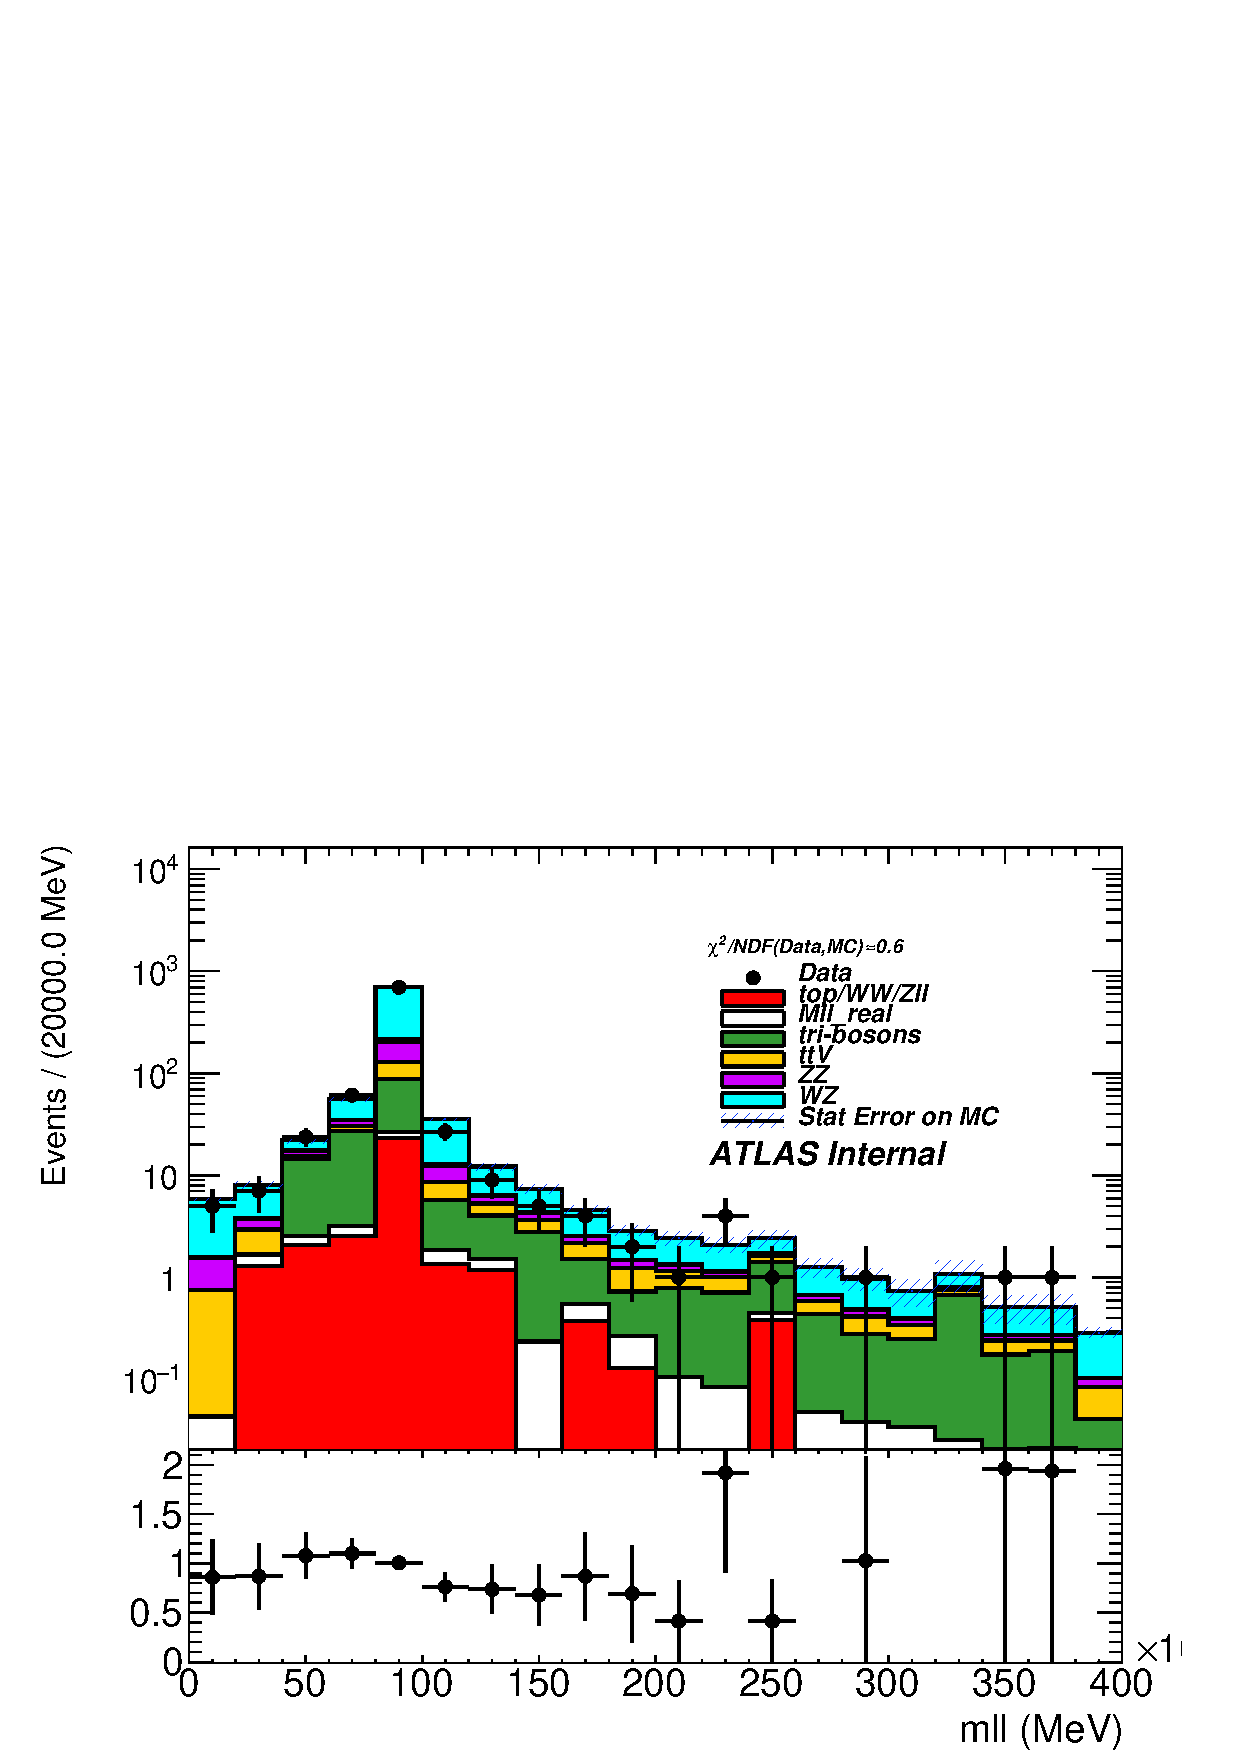
\includegraphics[width=0.45\textwidth]{figures/WZ_CR/2DSideband_WZCR_Isolated}
%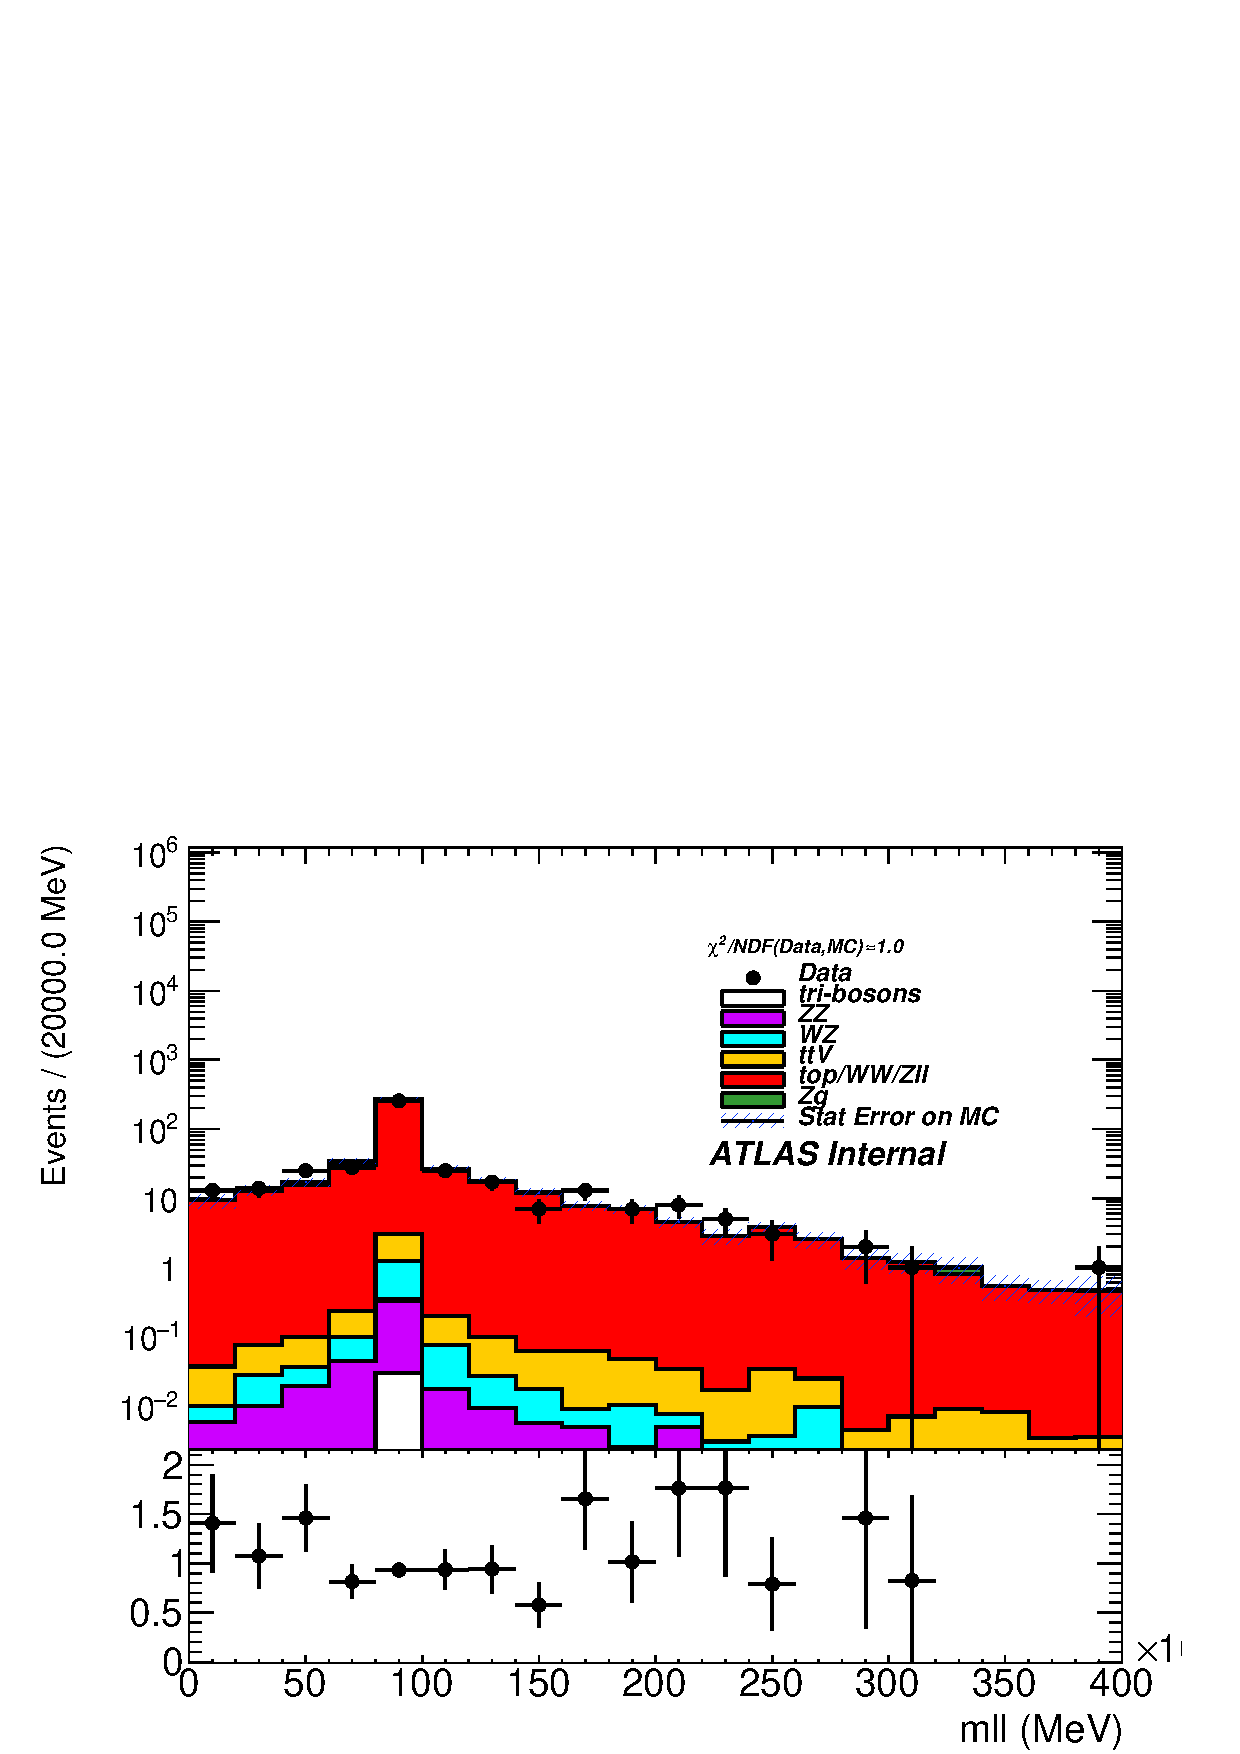
\includegraphics[width=0.45\textwidth]{figures/WZ_CR/2DSideband_WZCR_NonIsolated}
%\caption{ Distribution of $m_{\ell\ell}^{SFOS}$ in the isolated and  non-isolated 
%control regions. The agreement between the data and the MC expectation
%is not expected to be perfect, since the MC does not do a good job 
%of modeling the fake background. The 2D sideband method uses the data
%to estimate the fake background.}
%\label{fig:wz_sidebands}
%\end{figure}

The \z-veto and the isolation requirements are 
independently inverted\footnote{The thresholds are also slightly shifted 
so that there is a ``dead'' region between the signal regions and sidebands 
which is not used by either. This ensures separation between all regions.}
to form the three sidebands.
%The distribution of $m_{\textrm{SFOS}}$ is shown in
%\fig\ref{fig:wz_sidebands} in both the the isolated and non-isolated regions.
The expectation in each sideband can be parameterized
in the same way as \eqn\eqref{eq:wzparam}, resulting in one
equation for each region. By specifying the \z-veto condition
as $A$ and the isolation condition as $B$, \eqn\eqref{eq:wzparam}
can be rewritten as:
\begin{equation}
\label{eq:wzparam2}
N^{\textrm{Data}}_{A,B} =  N^{WZ}_{A,B} + N^{\textrm{Fake}}_{A,B} + N^{\textrm{Electroweak}}_{A,B}
\end{equation}
representing the four different equations after varying $A$ and $B$ independently.
For example, the signal region is when $A=\textrm{With \z-veto}$ and
$B=\textrm{Isolated}$.
One more equation can be found by assuming that the effect of 
the isolation cut on the fake background is independent of the \z-veto.
That is to say:
\begin{equation}
\label{eq:wz_constraint}
\frac{R^{\textrm{Fake}}_{\textrm{With \z-veto}}}{R^{\textrm{Fake}}_{\textrm{Without \z-veto}}} = K
\end{equation}
where 
\begin{equation}
R^{\textrm{Fake}}_{A} = 
\frac{N^{\textrm{Fake}}_{A,\textrm{Isolated}}}
{N^{\textrm{Fake}}_{A,\textrm{Non-Isolated}}}
\end{equation}
and it is assumed that $K=1$.
This results in five equations: the expectations,
\eqn\eqref{eq:wzparam2}, from varying the conditions $A$ and $B$ independently,
and \eqn\eqref{eq:wz_constraint}.




If we can solve the equations above for $N^{WZ}_{A,B}$ in the signal region,
when $A=\textrm{With \z-veto}$ and $B=\textrm{Isolated}$,
then we have our estimate. 
There are 5 equations and 16 unknowns. The four unknowns, $N^{\textrm{Data}}_{A,B}$,
are determined using the data directly while 
the electroweak backgrounds, $N^{\textrm{Electroweak}}_{A,B}$,
and the $WZ$ contributions in the sidebands, $N^{WZ}_{A,B}$ 
(when $A=\textrm{With \z-veto}$ and $B=\textrm{Isolated}$ are not both true)
are determined using $WZ$ MC. This reduces the problem to 5 equations
and 5 unknowns. Thus, we can solve algebraically for the remaining unknowns
including the desired value for the $WZ$ estimate in the signal region.

\begin{table}
\centering


\begin{tabular}{|cc|cc|}
\hline
%\multicolumn{3}{|c|}{$N^{\textrm{Data}}_{A,B}$}\\
\multirow{3}{*}{$N^{\textrm{Data}}_{A,B}$}&
\backslashbox{A}{B}& Isolated & Non-Isolated \\
\cline{2-4}
&With \z-veto & $724\pm27$ & $272\pm16$ \\
&Without \z-veto & $67\pm8$  & $118\pm11$ \\
\hline
\hline
%\multicolumn{3}{|c|}{$N^{\textrm{Electroweak}}_{A,B}$}\\
\multirow{3}{*}{$N^{\textrm{Electroweak}}_{A,B}$}&
\backslashbox{A}{B}& Isolated & Non-Isolated \\
\cline{2-4}
&With \z-veto & $172\pm3$ & $7.7\pm0.9$ \\
&Without \z-veto & $29\pm2$  & $1.9\pm0.6$ \\
\hline\hline
%\multicolumn{3}{|c|}{$N^{WZ}_{A,B}$ (MC)}\\
\multirow{3}{*}{$N^{WZ}_{A,B}$}&
\backslashbox{A}{B}& Isolated & Non-Isolated \\
\cline{2-4}
%&With \z-veto & $498\pm1$& $0.896\pm0.050$ \\
&With \z-veto & ---& $0.896\pm0.050$ \\
&Without \z-veto & $31.82\pm0.35$  & $0.095\pm0.015$ \\
\hline
\end{tabular}

\caption{All of the inputs used to constrain the system of five equations
from \eqn\eqref{eq:wzparam} and \eqn\eqref{eq:wz_constraint}.
The values are derived in the signal region and three sideband regions
described in the text. $N^{\textrm{Data}}_{A,B}$ are determined directly
from the data; $N^{\textrm{Electroweak}}_{A,B}$ and $N^{WZ}_{A,B}$ are 
determined in MC. The value for $N^{WZ}_{\textrm{With \z-veto,Isolated}}$ is
not used as an input and is instead solved for as the the main
parameter of interest. Still, the value is determined in MC to be
$498 \pm 1$.  Only statistical uncertainties are shown.}
\label{tab:wz_input}
\end{table}

\begin{table}
\centering


\begin{tabular}{|cc|cc|}
\hline
%\multicolumn{3}{|c|}{$N^{\textrm{Data}}_{A,B}$}\\
\multirow{3}{*}{$N^{\textrm{Fake}}_{A,B}$}&
\backslashbox{A}{B}& Isolated & Non-Isolated \\
\cline{2-4}
%&With \z-veto & $8\pm23$ &  \\ %this is the number provided by louis
&With \z& $14 \pm 43$ & $263\pm 16 $\\
&Without \z&  $6.2 \pm 8.3$ & $116 \pm 11$\\
\hline
\hline
\multirow{3}{*}{$N^{WZ}_{A,B}$}&
\backslashbox{A}{B}& Isolated & Non-Isolated \\
\cline{2-4}
&With \z& $537\pm35$ & --- \\ %I calculated 537.97 \pm 33.04
&Without \z& ---  & --- \\
\hline
\end{tabular}

\caption{Outputs from the system of five equations
from \eqn\eqref{eq:wzparam} and \eqn\eqref{eq:wz_constraint}
after including the numbers from \tab\ref{tab:wz_input} as input.
The value for $N^{WZ}_{\textrm{With \z-veto, Isolated}}$ is 
the value of primary interest.  Only statistical uncertainties are shown.}
\label{tab:wz_output}
\end{table}


The inputs to the system of equations are summarized in 
\tab\ref{tab:wz_input}\footnote{Note that the $WZ$ MC prediction in 
the signal region is not used except as a comparison.}.
The derived values after solving the system of equations are
summarized in \tab\ref{tab:wz_output}. 
The derived estimate for the $WZ$ contribution to 
the signal region is 
$537 \pm 35$
events, where the uncertainty is purely statistical. 
Compare this to the estimate from MC of 
$498 \pm 1$ events.
The ratio of the two can be used to derive a k-factor of
$1.08\pm0.07\stat$.


Systematic uncertainties are also derived on the method
by varying the 
thresholds used to define the sideband regions, varying the normalization
of the MC estimates in \tab\ref{tab:wz_input}, and by varying $K$ 
in \eqn\eqref{eq:wz_constraint} to match that observed in MC. The effect of each
uncertainty is propagated to the estimate of the $WZ$ normalization in
the signal region and are combined in quadrature. The total systematic
uncertainty is found to be 5.9\%. 
The final k-factor is thus $1.08 \pm0.07\stat\pm0.07\syst$.

The derived k-factor is applied to the MC estimate in another control
region enhanced in the $WZ$ process. This control region is determined
using the pre-selection region as described in \sec\ref{sec:preselection}
plus an additional requirement that there be 2 SFOS lepton pairs.
This gives a good test of the $WZ$ normalization in a control region
which is closer to the $WWW$ signal regions, but where the signal is still
suppressed since most of the signal region cuts are not applied.
The comparison is shown in \fig\ref{fig:WZ_2SFOS_CR} where
the data is shown to be in good agreement with the corrected $WZ$ MC
estimate, as desired.

\begin{figure}[htp]
\centering
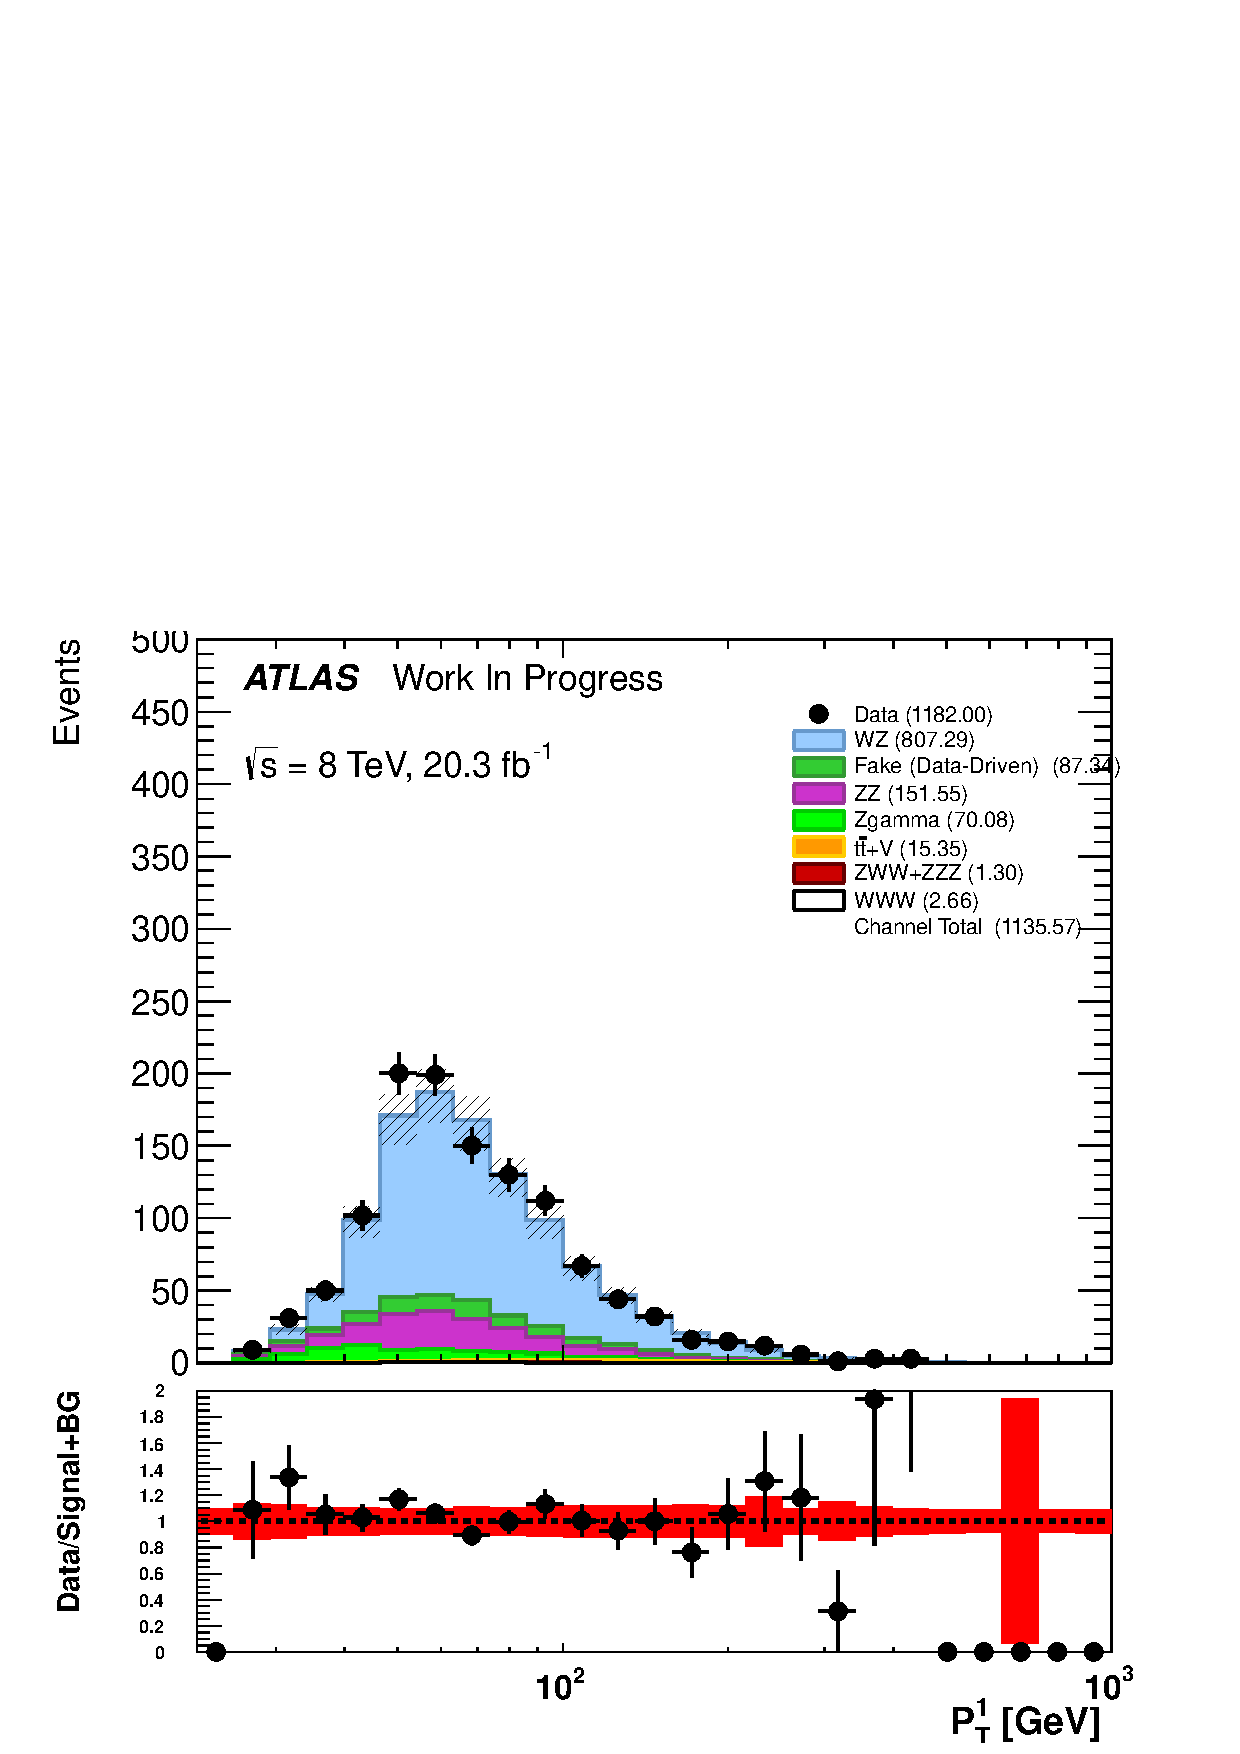
\includegraphics[width=0.4\textwidth]{figures/WZ_CR/LeadingLeptonPt_histratio.png}
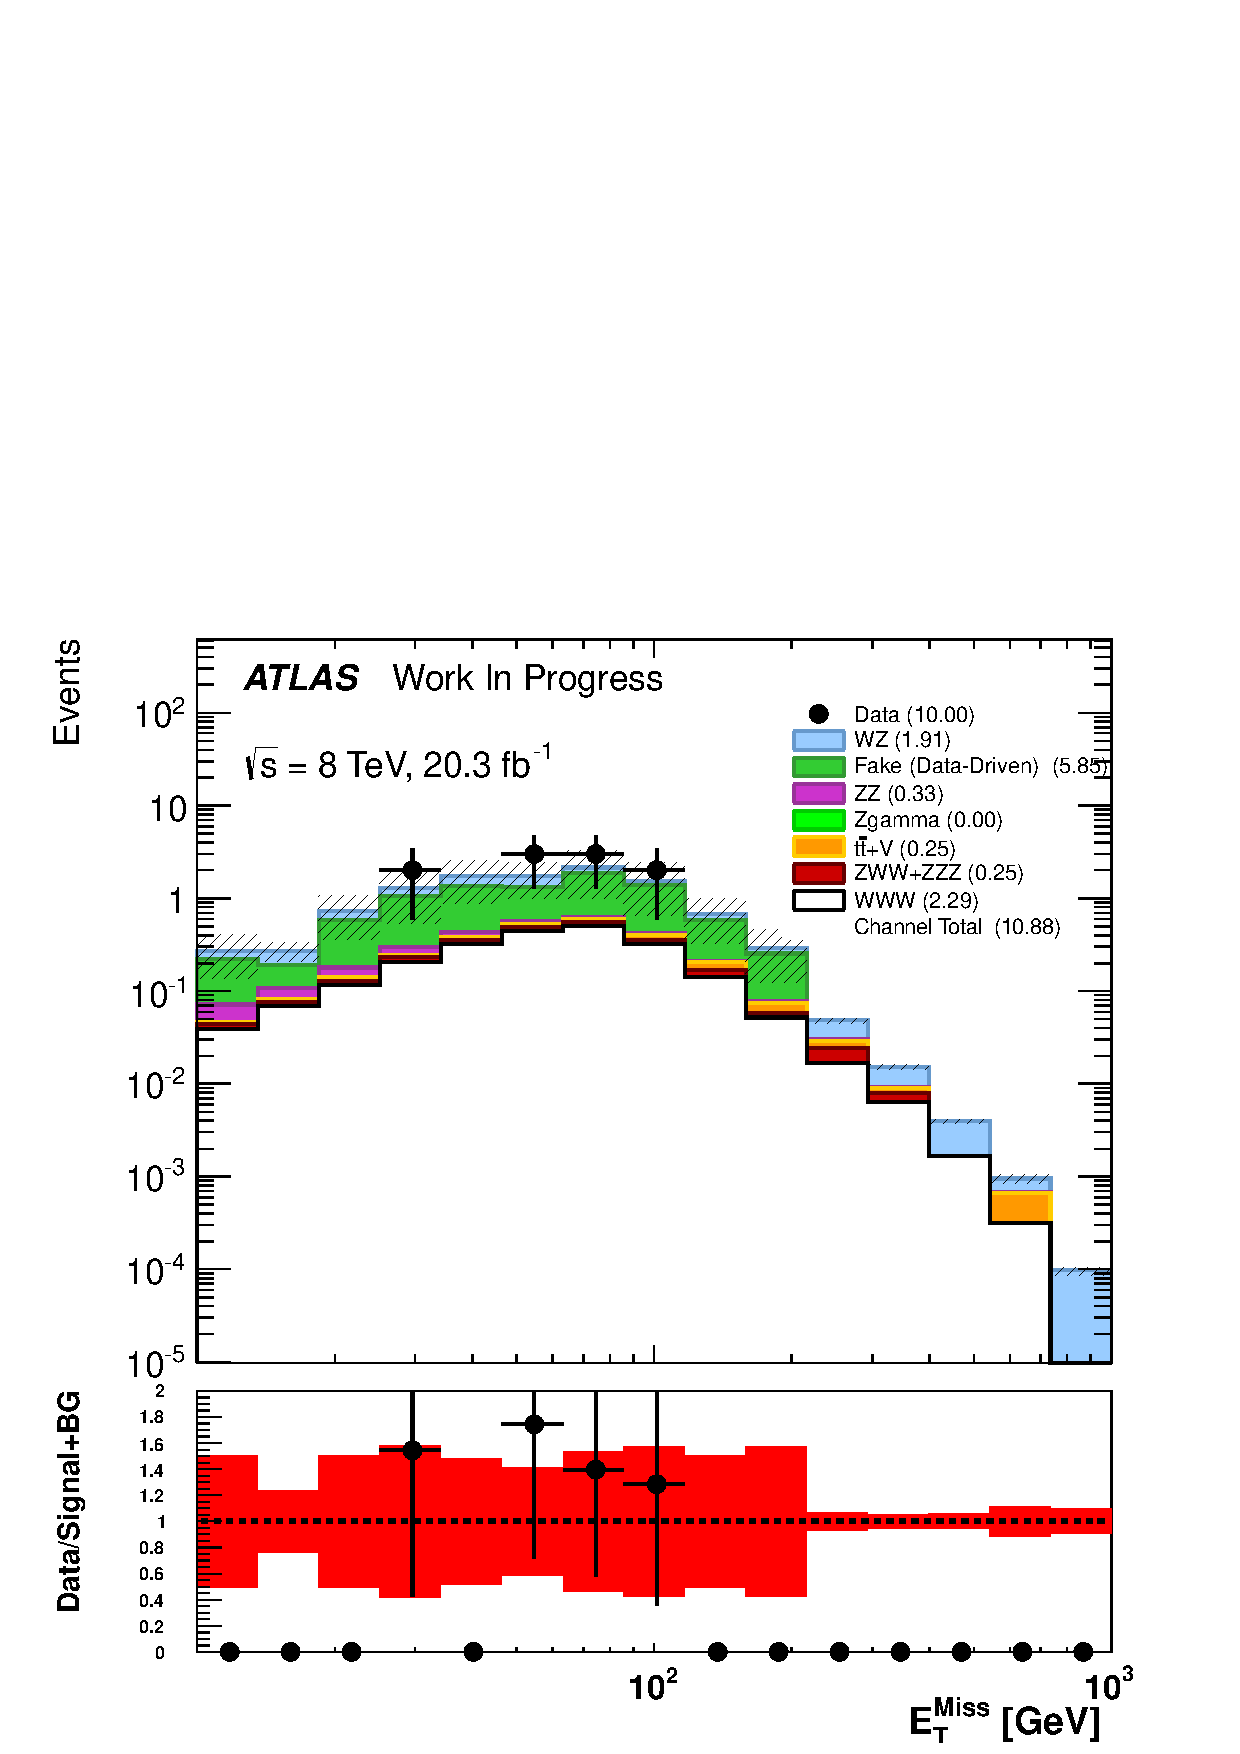
\includegraphics[width=0.4\textwidth]{figures/WZ_CR/MET_Et_histratio.png}
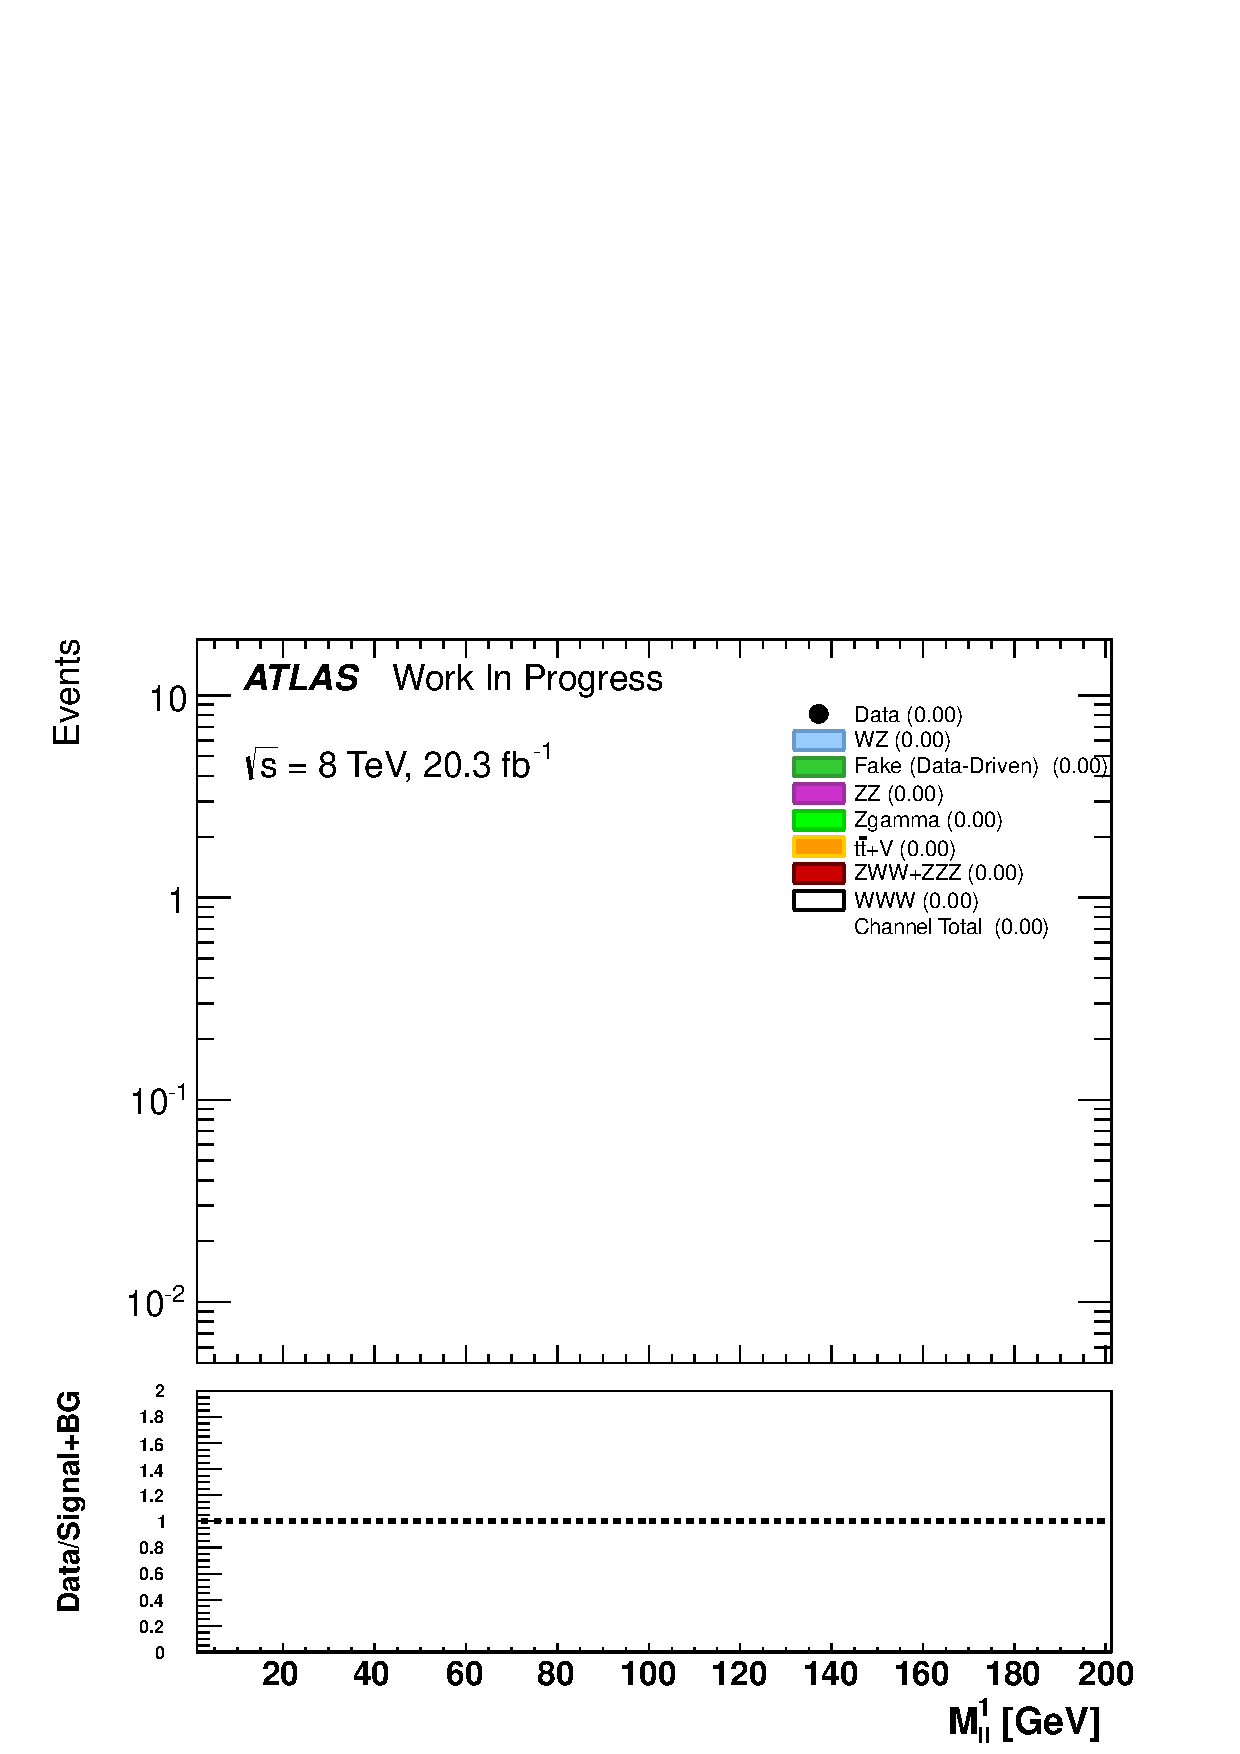
\includegraphics[width=0.4\textwidth]{figures/WZ_CR/InvariantMassSFOS_histratio.png}
\includegraphics[width=0.4\textwidth]{figures/WZ_CR/NJets_histratio.png}
\caption{$WZ$ control region with 3 lepton pre-selection plus 2 SFOS requirement. 
Distributions show leading lepton $p_{T}$, $\MET$, $m_{12}$, and jet multiplicity. 
The systematic band shows the uncertainty on the $WZ$ k-factor.}
\label{fig:WZ_2SFOS_CR}
\end{figure}  

As a further test of the method, a MC estimate which includes the $WZ$ signal as
well as the electroweak and fake backgrounds is used as input in place 
of $N^{\textrm{Data}}_{A,B}$ to see if the MC estimate for the $WZ$
contribution in the signal region can be recovered. This is referred to as
a closure test.  The measured value for the $WZ$ normalization from the 
closure test is found to be  $495\pm39$, which is indeed consistent with the
estimate from pure MC of $498\pm1$. The closure test also shows consistent
results when varying the normalizations of the different components 
in the MC independently.




\subsubsection{$ZZ\rightarrow llll$}
\label{sec:zzbg}

The $ZZ\rightarrow llll$ process has a similar cross-section as 
the $WZ\rightarrow lll\nu$ process but is 
suppressed by the probability that exactly one lepton is not reconstructed. 
Still, this probability is large enough that the $ZZ$ background is one of the 
largest in the 1 and 2 SFOS signal regions.  
Unlike the $WZ$ process, NNLO predictions are available 
from~\cite{Cascioli:2014yka,Baglio:2013toa,Bierweiler:2013dja}
that suggest a k-factor of 1.05 on the overall $ZZ$ prediction.
The uncertainty on the prediction is determined to be 
15\%~\cite{Cascioli:2014yka,Baglio:2013toa,Bierweiler:2013dja}.
This correction is used instead of determining a correction in the data
like in \sec\ref{sec:wzbg}.

We may check how well the NLO $ZZ\rightarrow llll$ MC prediction and 
NNLO normalization correction describe the process in the data by looking
in a four lepton control region. The reconstructed leptons are required to have
the same quality requirements as in \sec\ref{sec:object_selection}.
The leptons are sorted by \pt~with the highest \pt~lepton
required to have $\pt>25\GeV$, the next two to have
$\pt>15\GeV$, and the lowest \pt~lepton to have $\pt>10\GeV$.
From these leptons, two separate SFOS pairs are formed. If there
is any ambiguity, first an SFOS pair is formed which gives the greatest
possible di-lepton invariant mass and the remaining leptons form the other pair.
This is a similar procedure to~\cite{Aad:2014wra}. Finally, 
to suppress background contamination in the control region,
the invariant mass of both SFOS pairs are required to be near the \z-mass, 
with $60\GeV<m_{\textrm{SFOS}}<120\GeV$ for both.
The results of the comparison are summarized for a few different distributions
in \fig\ref{fig:ZZ_CR} and on the total yield in \tab\ref{tab:ZZ_CR}.
The expectation is shown to agree well with the observed data within the 
stated systematic uncertainty on the k-factor of 15\%. 


%%%%Should I say anything about this off shell business? Probably not.
%It was also checked whether or not the contribution of $ZZ^{*}$ where 
%the $Z^{*}$ boson is very off-shell, $m_{Z^{*}} < 4$~GeV, while the other boson
%has a  mass $m_Z > 4$~GeV has any impact on the signal regions. This was 
%evaluated by looking at the samples with channel numbers
%$181471$ through $181479$ in Table~\ref{tab:sample_bkg_dibosons}.  
%The contribution from these samples were found to be negligible, with a 
%statistical uncertainty compatible with exactly 0 events in the individual 
%signal regions. As a result, these samples were not considered any further 
%and are not included in the final background  estimate for the signal regions 
%or in the ZZ control regions.


\begin{figure}[htp]
\centering
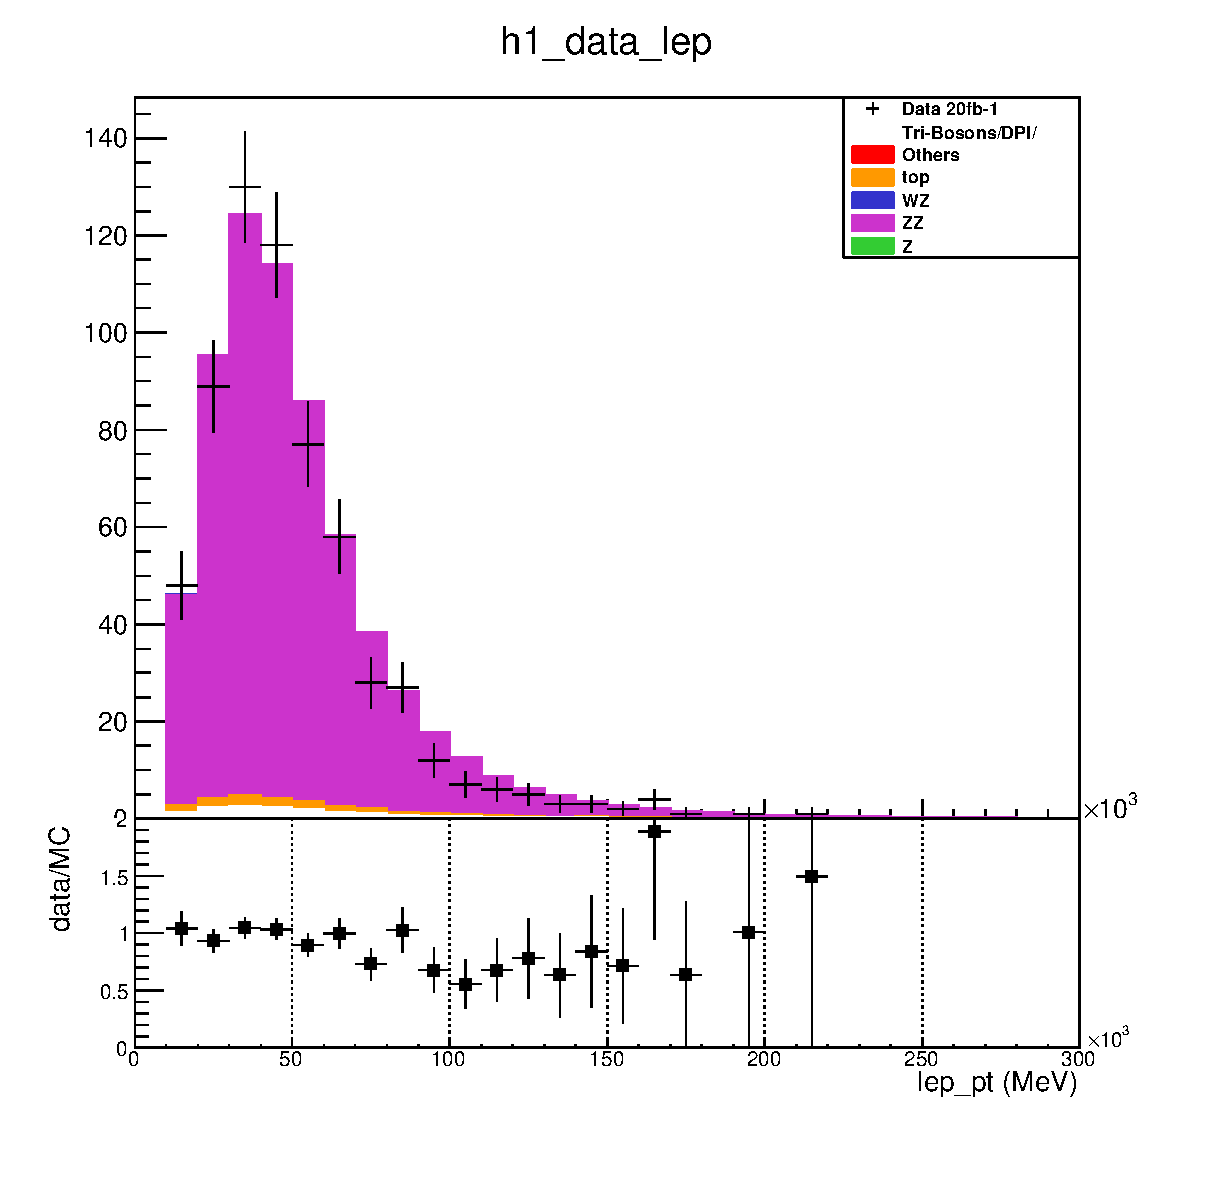
\includegraphics[width=0.4\textwidth]{figures/ZZ_CR/ZZ_CR_lep_pt.eps}
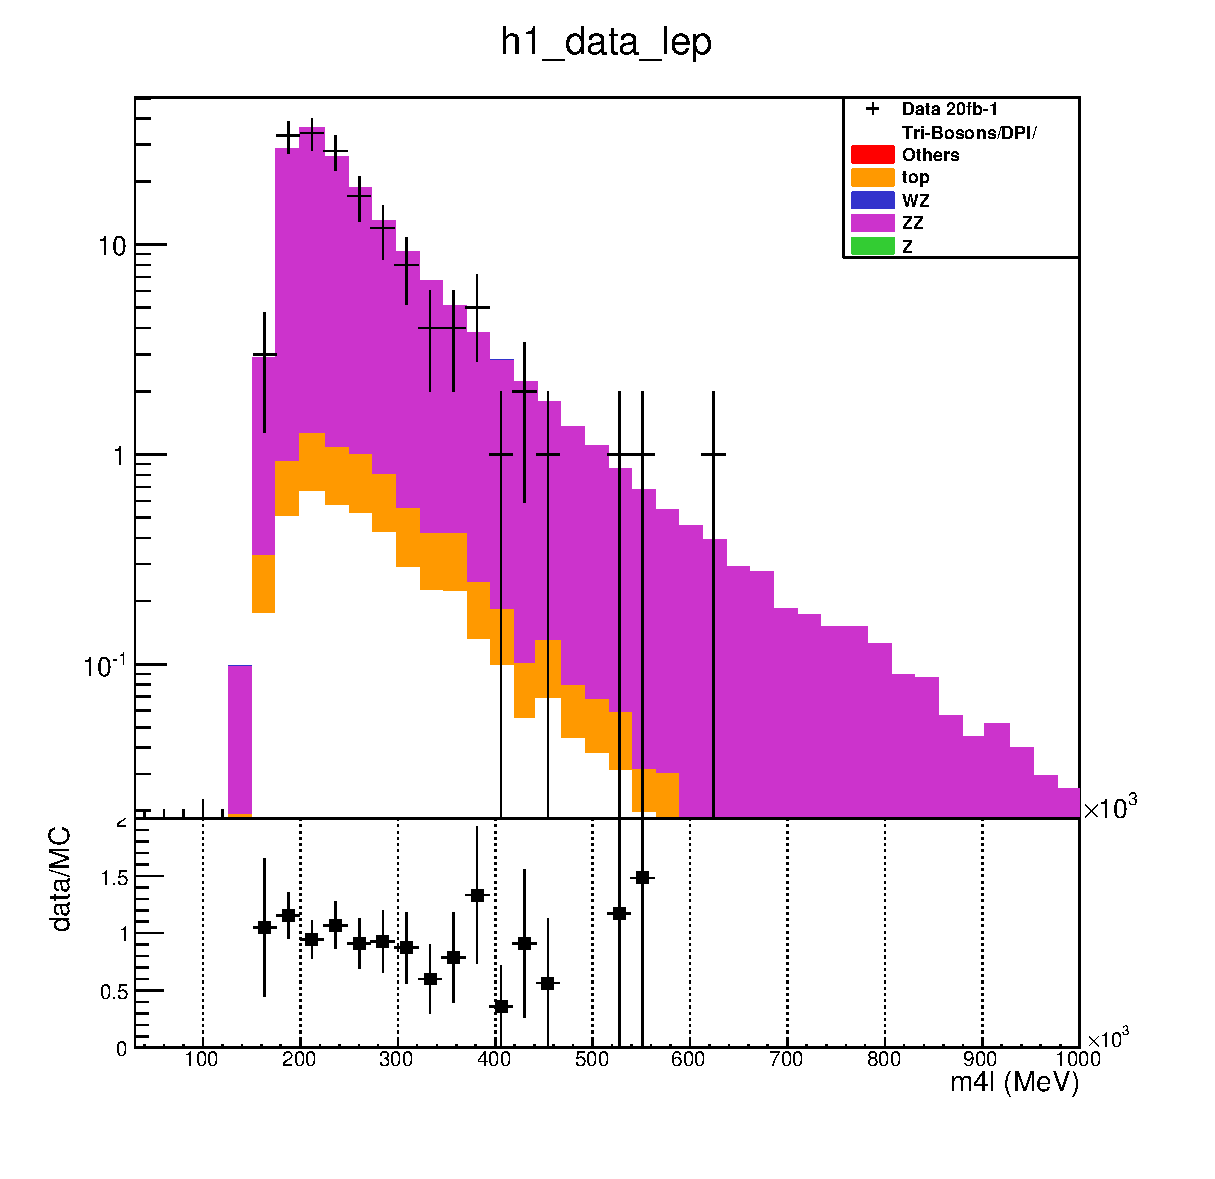
\includegraphics[width=0.4\textwidth]{figures/ZZ_CR/ZZ_CR_m4l.eps}
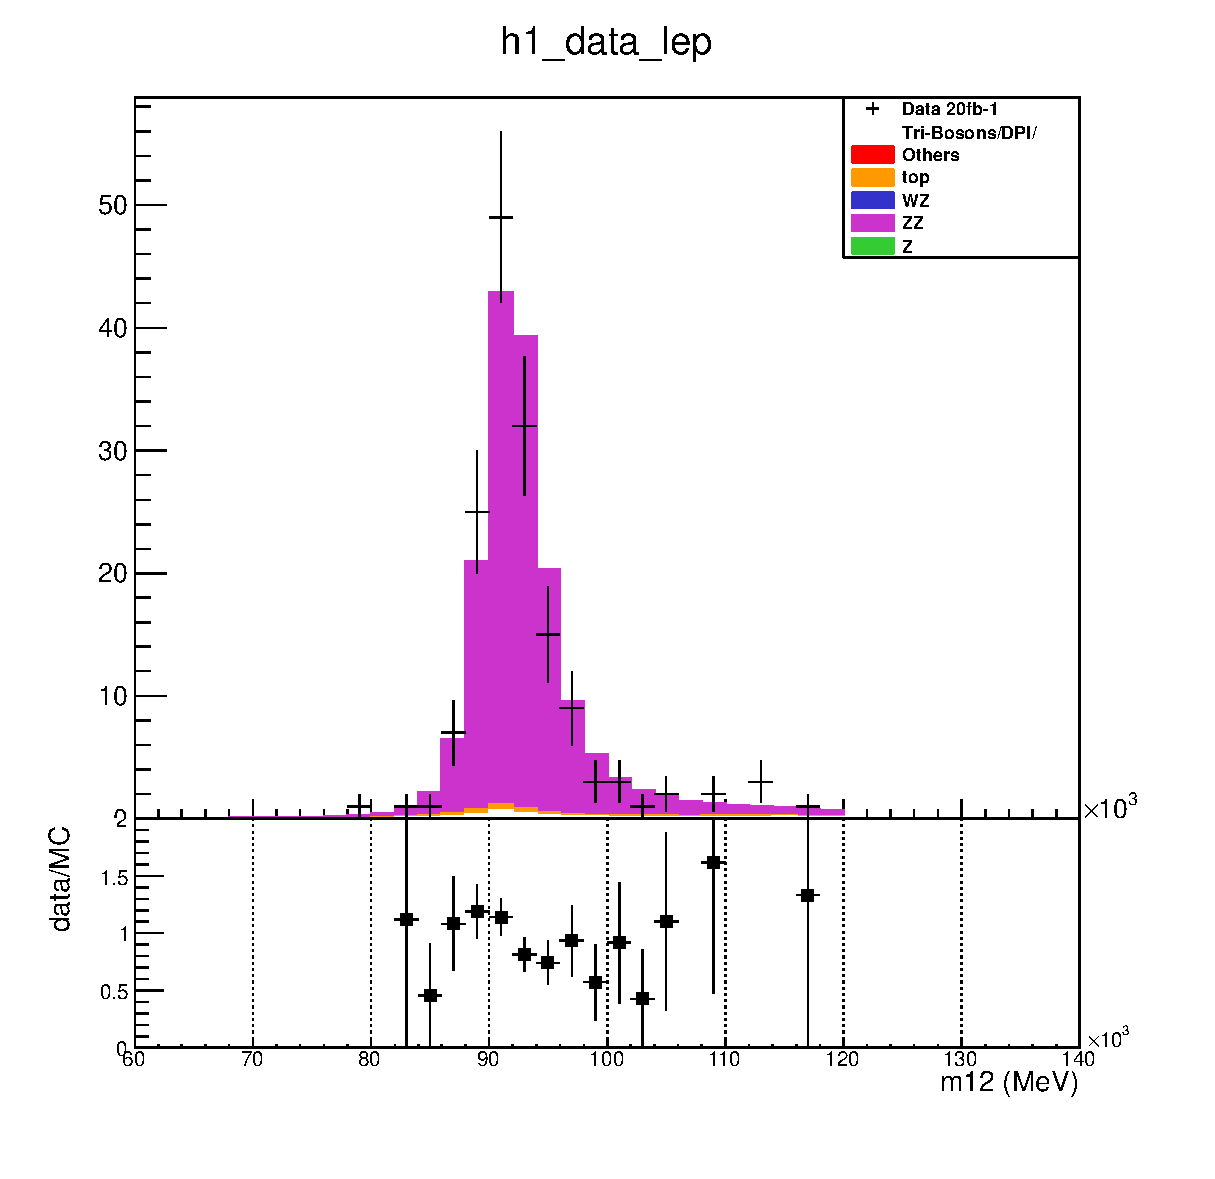
\includegraphics[width=0.4\textwidth]{figures/ZZ_CR/ZZ_CR_m12.eps}
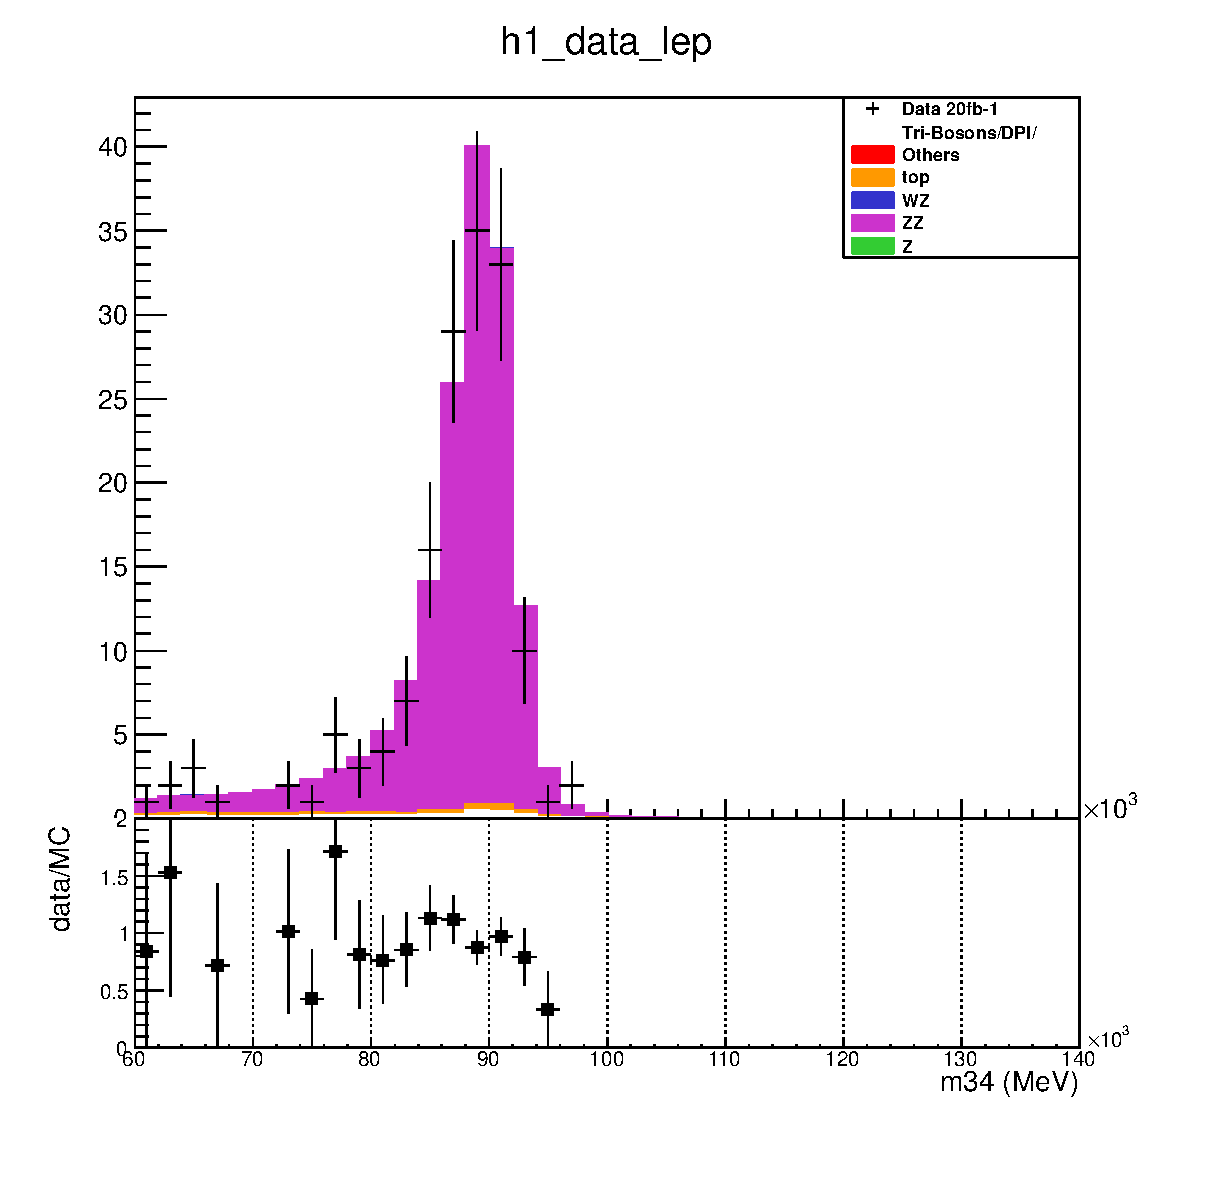
\includegraphics[width=0.4\textwidth]{figures/ZZ_CR/ZZ_CR_m34.eps}

\caption{$ZZ\rightarrow llll$ control region with two separate SFOS pairs. 
Distributions are shown for the lepton \pt, the leading di-lepton mass ($m_{12}$), 
the minimum di-lepton mass ($m_{34}$), and the four lepton mass ($m_{4l}$).}
\label{fig:ZZ_CR}
\end{figure}  

\begin{table}[htp]
\centering
\begin{tabular}{|c||c|c|c|c|}
\hline
 & Event Yield\\ 
\hline\hline
$WZ$ &  $0.05 \pm 0.01$\\ 
$ZZ$ &  $156.2 \pm 0.3$(stat) $\pm 22.3$(syst) \\ 
% $gg2ZZ$ &	$21.3 \pm 0.2$ \\
$Z\gamma$ &  $0.0 \pm 0.0$\\ 
Fake (MC) &  $3.6 \pm 0.2$\\ 
tri-boson and $t\bar{t}+V$ &  $4.1 \pm 0.2$\\ 
\hline
Expected Signal + Background &  $164.0 \pm 0.3$ (stat) $\pm 22.3$(syst)\\ 
\hline
Observed Data &  $155$\\ % \pm 12$\\ 
\hline
\end{tabular}
\caption{Number of data and predicted events in the $ZZ$ control region. 
The error quoted on the MC samples, except for $ZZ$,
represents only the statistical error. 
The systematic error due to the k-factor on the $ZZ$ sample is also shown.}
\label{tab:ZZ_CR}
\end{table}



\subsubsection{$Z\gamma$}
\label{sec:zgammabg}

The $\z\gamma$ process can produce three leptons and thus falls into the 
signal regions.
Measurements of this process within ATLAS
have shown that this process is well described by MC simulation
using the \sherpa~generator at both 7 and 8~\TeV~\cite{Aad:2013izg,Auerbach:1631102}.
Thus, no further correction or uncertainty on the normalization is applied.

The description of the $\z\gamma$ process is tested in a three lepton control
region starting from the 
pre-selection (described in \sec\ref{sec:preselection}) and with the same
lepton quality requirements as in \sec\ref{sec:object_selection}.
One of the three leptons should be an electron while the remaining two 
are required to form a di-muon SFOS pair. For this final state to be produced
by the $\z\gamma$ process, the electron should always come from 
pair production off of the photon, $\gamma$, which itself radiates
off of the initial state \z~boson.  As a result, the invariant mass
of the di-muon pair coming from the \z-decay will typically be shifted
slightly below the \z-mass. However, the invariant mass of the three lepton 
system should restore this shift such that the mass peak is again centered 
on the \z-mass. Thus, in order to further suppress backgrounds to the 
$\z\gamma$ process, we also require that the three-lepton invariant
mass, $m_{\mu\mu e}$, be within 15~\GeV of the \z-mass.
The prediction after this selection is compared to data for a few different
distributions in \fig\ref{fig:Zgamma_CR} and for the total yield
in \tab\ref{tab:Zgamma_CR}. The control region is clearly enhanced
in the $\z\gamma$ process, and furthermore shows very good agreement. 
This is even true for distributions of the electron kinematics, 
such as $\eta$ and $\pt$, which suggests that the photon conversion
mechanism is being well modeled.

\begin{figure}[htp]
\centering
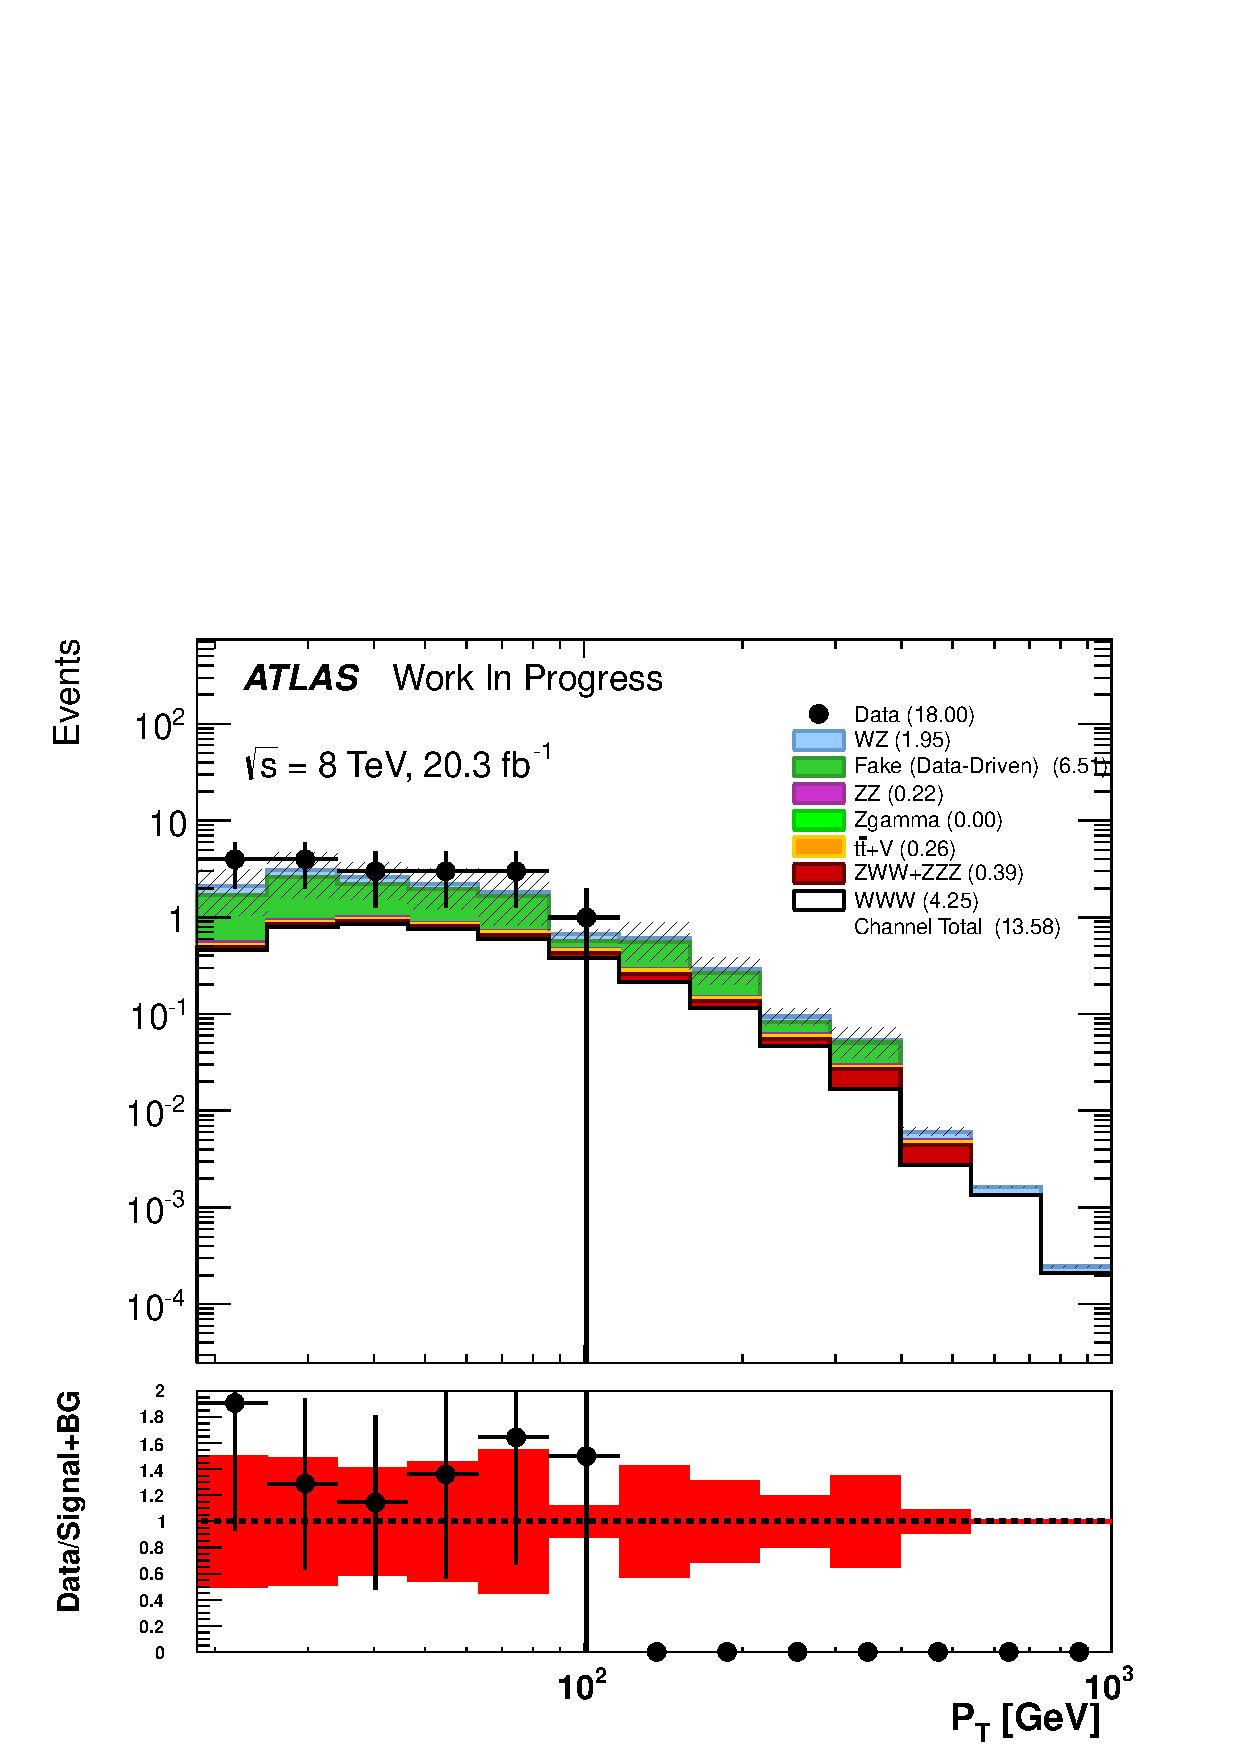
\includegraphics[width=0.4\textwidth]{figures/ZG_CR/AllLeptonPt_histratio.png}
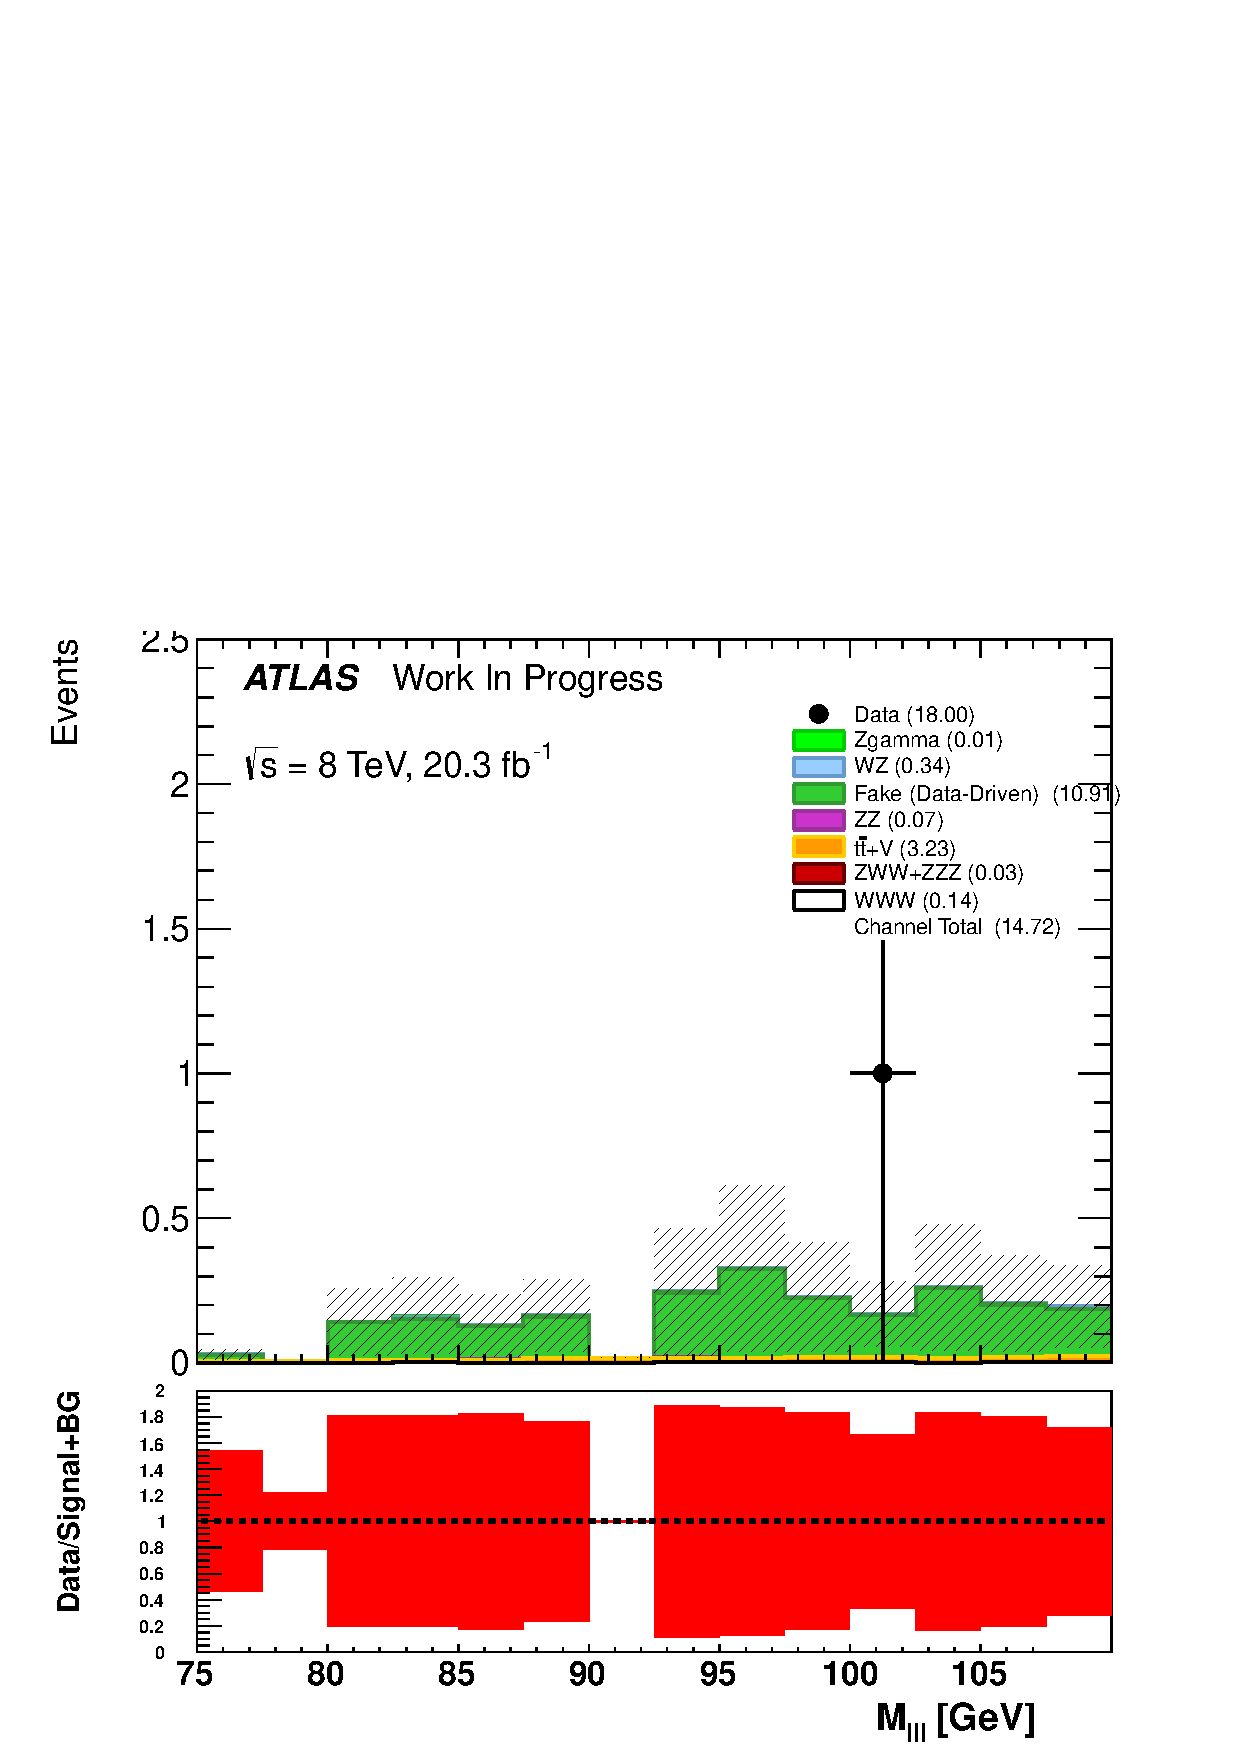
\includegraphics[width=0.4\textwidth]{figures/ZG_CR/InvariantMassThreeLep_histratio.png}
\includegraphics[width=0.4\textwidth]{figures/ZG_CR/ElectronEta_histratio.png}
\includegraphics[width=0.4\textwidth]{figures/ZG_CR/NJets_histratio.png}

\caption{Three lepton $Z\gamma$ control region. Distribution are shown for the
lepton $p_{T}$, three lepton invariant mass ($m_{\mu\mu e}$), electron $\eta$, 
and jet multiplicity.}
\label{fig:Zgamma_CR}
\end{figure}  


\begin{table}[ht!]
\centering
\begin{tabular}{|c||c|c|c|c|}
\hline
 & Event Yield\\ 
\hline\hline
$WZ$ &  $7.47 \pm 0.11$\\ 
$ZZ$ &  $9.116 \pm 0.075$\\ 
$Z\gamma$ &  $80.3 \pm 2.8$\\ 
$ZWW+ZZZ$ &  $0.0285 \pm 0.0046$\\ 
$t\bar{t}+V$ &  $0.338 \pm 0.012$\\ 
Fake (data-driven) &  $21.9 \pm 1.2$\\ 
$WWW$ &  $0.3142 \pm 0.0072$\\ 
\hline
Expected Background &  $119.2 \pm 3.1$\\ 
Expected Signal + Background &  $119.5 \pm 3.1$\\ 
\hline
Observed Data &  $119$\\ 
\hline
\end{tabular}

\caption{Expected and observed event yields for the Z$\gamma$ control region. 
Only statistical uncertainties are shown.}
\label{tab:Zgamma_CR}
\end{table}



\subsubsection{Other Monte Carlo Backgrounds}
\label{sec:otherbg}


Backgrounds due to DPS are generated using MC as described
in \sec\ref{sec:www_bg_samples}. The cross-section of the DPS process
is calculated assuming that the cross-sections of the two incoming processes
can be factorized as in \cite{Gaunt:2010pi} using an effective
proton cross-section measured in ATLAS at 7~\TeV~\cite{Aad:2013bjm}.
An overall 50\% uncertainty is placed on the normalization of these cross-sections.
This is a conservative estimate of the uncertainty.
However, the contributions of these processes are found to be negligible.
%citation on the uncertainty?


The remaining backgrounds evaluated using MC are those containing 
at least three real leptons but whose cross-sections are small or on 
the order of the signal process, namely $\ttV$ and $VVV$ processes.
The theory uncertainties on the $\ttV$ normalization have been found by
ATLAS to be about 30\% and have been shown to give a 
consistent prediction~\cite{ATLAS-CONF-2015-032}. 
%do I also need to cite a twiki for this 30% uncertainty
%look at this conf note.
An uncertainty of 30\% is also assigned to the normalization of the 
$VVV$ samples.
